%%
%  ******************************************************************************
%  * #file    Szablon_raportu_EN_Latex.tex
%  * #author  Adrian Wójcik   adrian.wojcik(at)put.poznan.pl
%  *          
%  * #commit  Patryk Kościk   koscikpatryk(at)gmail.com
%  *          Modified the template for Projekt przejsciowy purposes          
%  *          
%  * #version 1.0
%  * #date    09-Mar-2022
%  * #brief   PROJPRZEJ
%  *
%  ******************************************************************************
%%  
\documentclass[11pt, a4paper]{article}

\usepackage{SM_template}

% Wypełnijcie te dyrektywy zgodnie z waszym tematem
% \lab      -> NAZWA CZUJNIKA, np.: 'DHT22'
% \comment  -> Króciutki opis co to, np.: 'Cyfrowy budżetowy czujnik temperatury'
%
\lab{Moduł KY-031}
\comment{Cyfrowy czujnik do wykrywania stuknięć}

% Absolutny zakaz dotykania tego tutaj bo jak dotkiecie to coś jebnie
\university{Politechnika Poznańska}
\faculty{Wydział Automatyki, Robotyki i Elektrotechniki}
\institute{Instytut Robotyki i Inteligencji Maszynowej}
\department{Zakład Sterowania i Elektroniki Przemysłowej}
\addbibresource{bib/nazwa-modulu.bib}
\nocite{*}


%%
%
% Początek dokumentu
%
%%
\begin{document}

%% Strona tytułowa %%
\mainpage{{KY-031/KY-031.jpeg}}
\newpage

\section*{Opis elementu} \addcontentsline{toc}{section}{Wstęp}
Czujnik KY-031 składa się ze sprężynowego sensora, wbudowanego rezystora 10k $\Omega$ i 3 męskich pinów. Sprężyna emituje sygnał wysoki w momencie wyczucia wibracji. 

\vspace{0.5cm}
\begin{figure}[h]
\centering
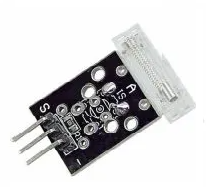
\includegraphics[scale=0.5]{fig/KY-031/zdj_modułu/fig1.png}
\caption{Moduł KY-031}
\label{fig:sub1}
\end{figure}
\vspace{0.5cm}

\subsection{Zasada działania}
Budowę czujnika widzimy na rysunku poniżej. W momencie dojścia wibracji/stuknięć do czujnika, sprężyna na górze modułu wysyła sygnał wysoki, co oznacza wykrycie danego zdarzenia.

\vspace{0.5cm}
\begin{figure}[h]
\centering
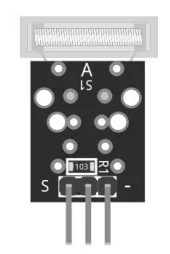
\includegraphics{fig/KY-031/zasada_dzialania/fig2.png}
\caption{Poglądowy rysunek modułu}
\label{fig:sub1}
\end{figure}
\vspace{0.5cm}

\subsection{Zastosowania}
Czujniki stuknięć są szeroko wykorzystywane przy silnikach. Dzięki odpowiedniu zaimplementowaniu takiego modułu jesteśmy w stanie wpłynąć zmniejszenie spalania w samochodzie i zwiększenie momentu obrotowego.

\newpage

\section{Implementacja czujnika}
Ogólny schemat elektryczny modułu KY-031 został przedstawiony poniżej.

\subsection{Połączenie fizyczne}

\vspace{0.5cm}
\begin{figure}[h!]
    \centering
    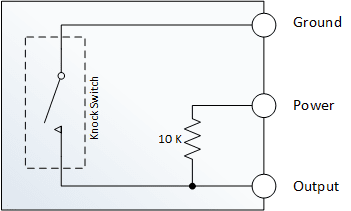
\includegraphics[scale=0.75]{fig/KY-031/polaczenie_modulu/polaczenie.png}
    \caption{Schemat modułu}
    \label{fig:my_label}
\end{figure}
\vspace{0.5cm}

\vspace{0.5cm}
\begin{table}[h!]
    \centering
    \begin{tabular}{|c|c|c|c|} 
        \hline
        \multicolumn{2}{|c|}{NUCELO-L476RG} & \multicolumn{2}{c|}{SENSOR}  \\ 
        \hline
        Etykieta & Port i numer pinu       & Nr pinu & Etykieta           \\ 
        \hline
        S        & CN8 - A1                        & 1       & Output                 \\
        5V       & CN6 - 5                   & 2       & Power              \\
        GND      & -                       & 3       & Gnd              \\
        
        \hline
    \end{tabular}
    \caption{Połączenie czujnika z mikrokontrolerem}
\end{table}
\vspace{0.5cm}

\newpage

\subsection{Kongiuracja IOC}
Mikrokontroler skonfigurowano w środowisku CubeID.

\vspace{0.5cm}
\begin{figure}[h!]
    \centering
    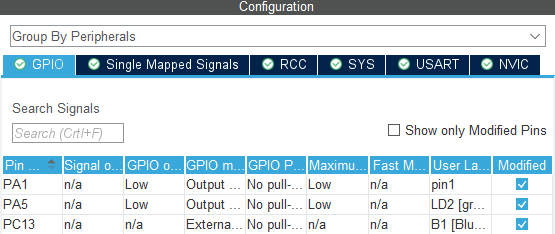
\includegraphics[width=9cm]{fig/KY-031/polaczenie_modulu/confIOC.png}
    \caption{Konfiguracja GPIO}
    \label{fig:my_label}
\end{figure}
\vspace{0.5cm}

\subsection{Oprogramowanie mikrokontrolera}
Kod obsługujący moduł znajduję sie w suplemencie umieszczonym pod koniec rozdziału.

\section{Prezentacja działania układu}
Prezentacja złożonego układu z wgranym programem.

\vspace{0.5cm}
\begin{figure}[h!]
    \centering
    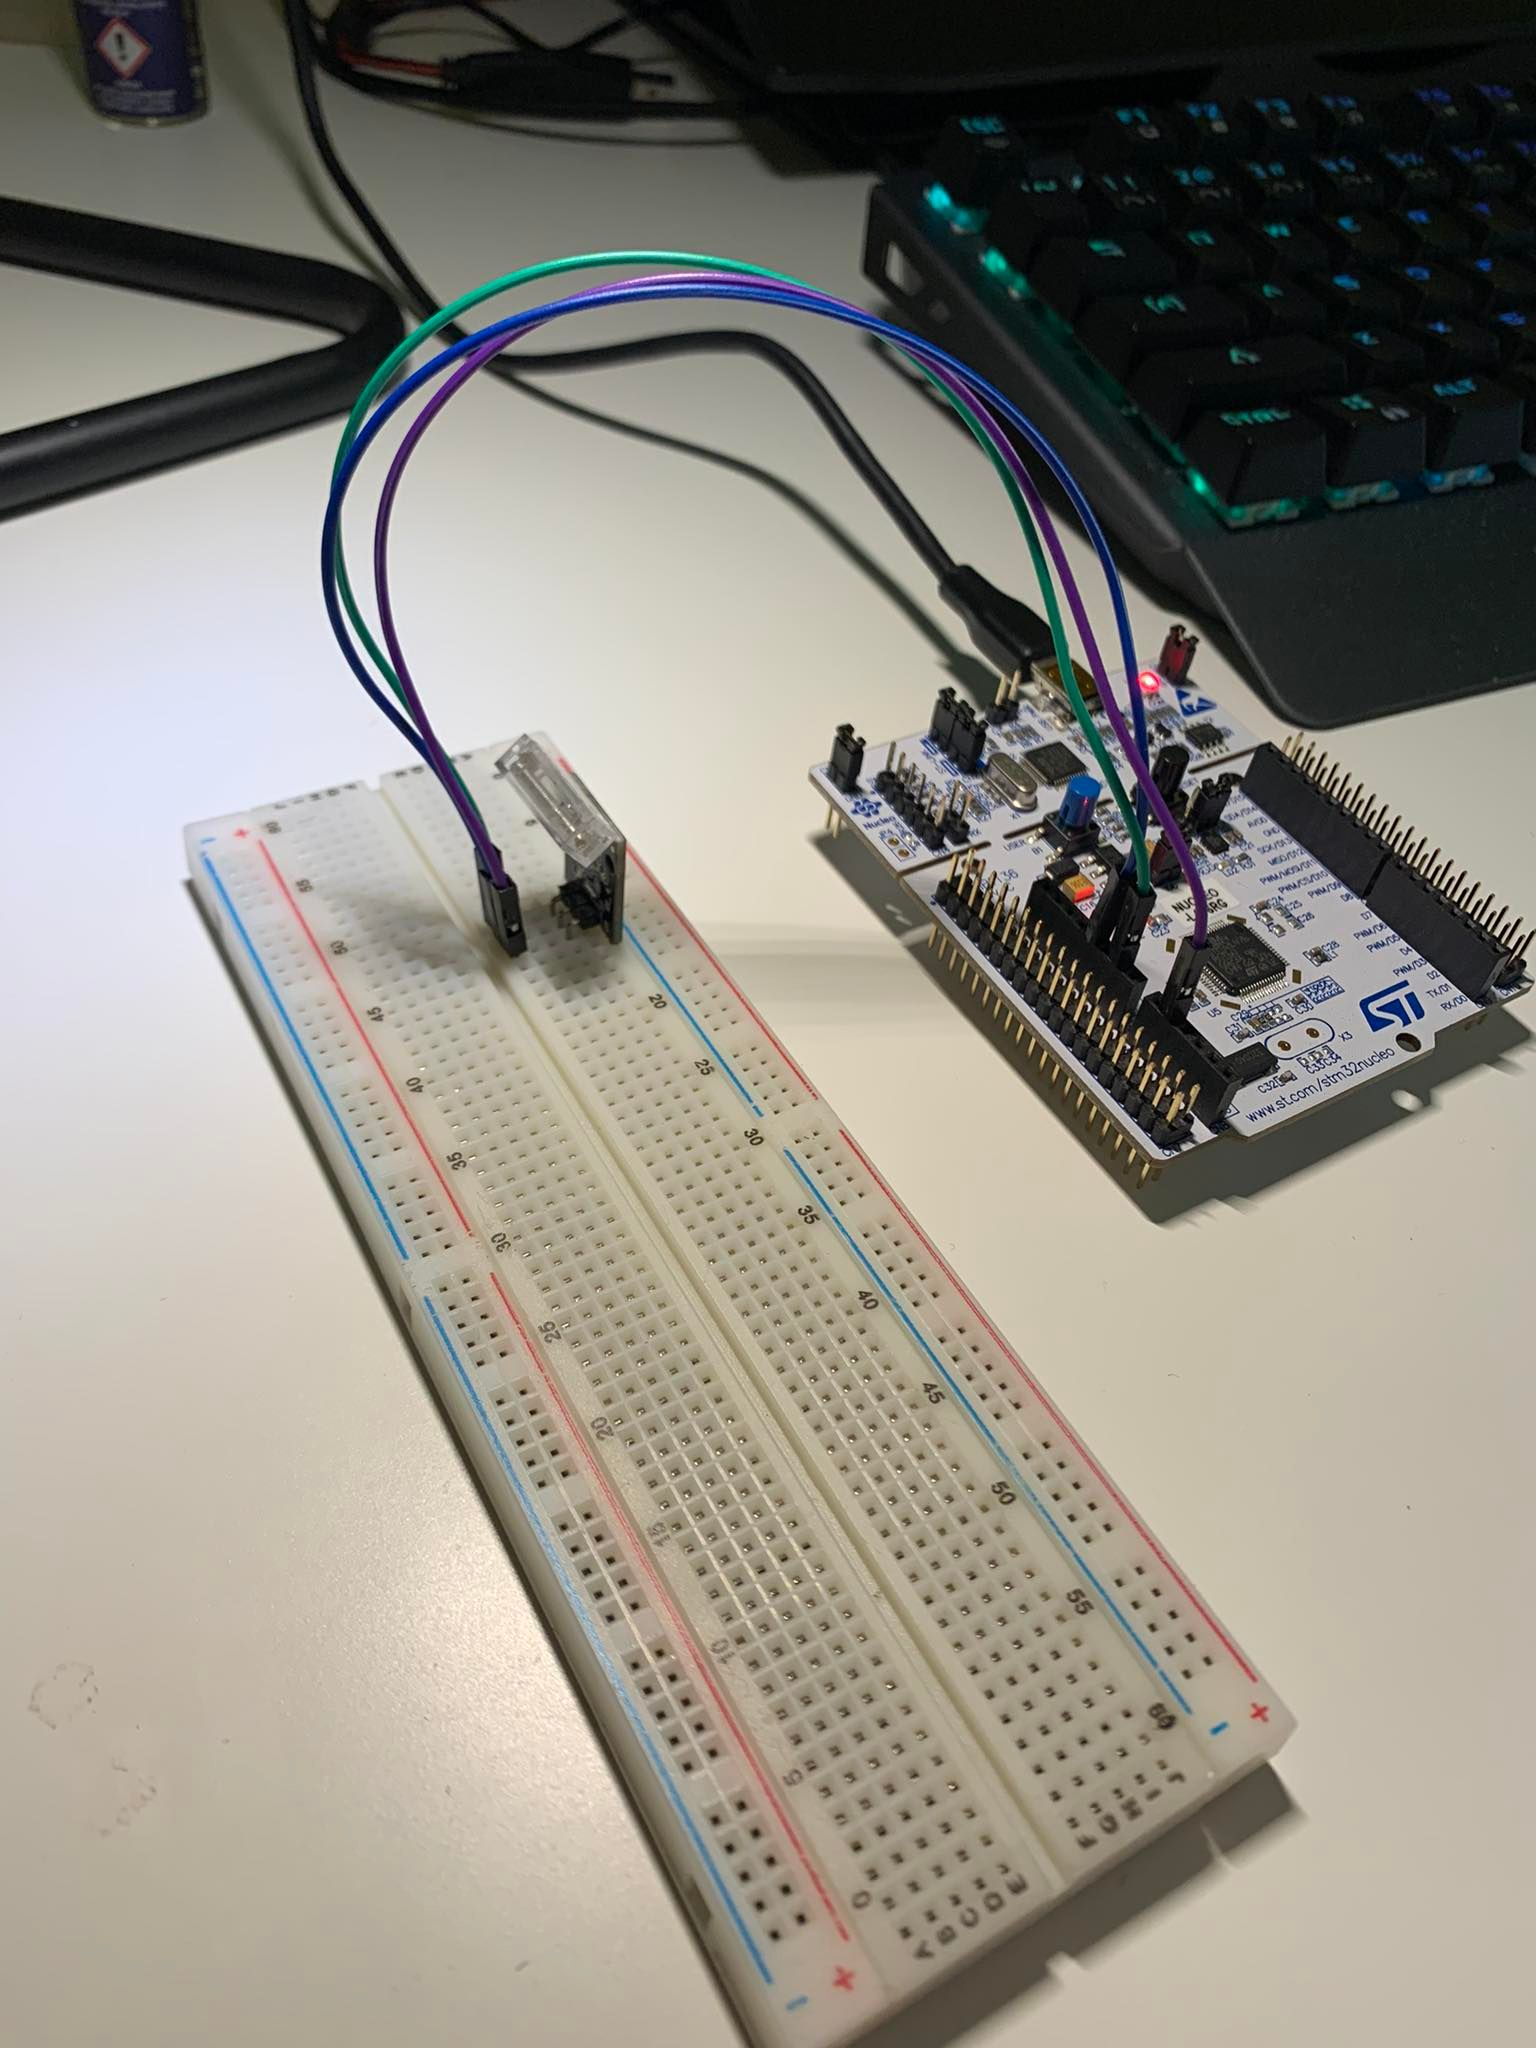
\includegraphics[scale=0.1]{fig/KY-031/działanie_ukladu/uklad.jpg}
    \caption{Złożony układ modułu KY-031}
    \label{fig:my_label}
\end{figure}
\vspace{0.5cm}

\end{document}